\begin{flushright} {\tiny {\color{gray} (tikz\_staggered2D\_divv.tex)}} \end{flushright}
%~~~~~~~~~~~~~~~~~~~~~~~~~~~~~~~~~~~~~~~~~~~~~~~~~~~~~~~~~~~~~~~~~~~~~~~~~~~~~~~~~~~~~~~~~~~~~~~~~~


\begin{center}
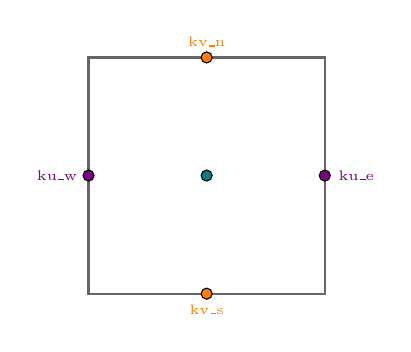
\begin{tikzpicture}
%\draw[fill=gray!23,gray!23](0,0) rectangle (5,5);
%\draw[step=0.5cm,gray,very thin] (0,0) grid (5,5); %background grid
\draw[thick,black!60] (1,1) -- (4,1) -- (4,4) -- (1,4) -- cycle ; 
\draw[black,fill=teal] (2.5,2.5)   circle (2pt);
%---------------------------------------------------
\node[] at (2.5,0.8) {\tiny \color{orange} kv\_s};
\node[] at (2.5,4.2) {\tiny \color{orange} kv\_n};
\draw[black,fill=orange] (2.5,1)   circle (2pt);
\draw[black,fill=orange] (2.5,4)   circle (2pt);
%---------------------------------------------------
\node[] at (0.6,2.5) {\tiny \color{violet} ku\_w};
\node[] at (4.4,2.5) {\tiny \color{violet} ku\_e};
\draw[black,fill=violet] (1,2.5)   circle (2pt);
\draw[black,fill=violet] (4,2.5)   circle (2pt);
\end{tikzpicture}
\end{center}


